We shall now present a representation of the problem which will greatly simplify the analysis of $v$ and $h$ collisions for some ball $b$, called the tiling representation. First we will define some basic definitions we need to explain the tiling representation.

\begin{definition}
  A billiard ball \emph{trajectory} $\tau(t_0, t_1)$ is the curved traced by a billiard ball $b$ between times $t_0$ and $t_1$.
\end{definition}

\begin{definition}
  A collision time $\kappa_i$ for a billiard ball $b$ is the time at which the $i$th collision occurs.
\end{definition}

To understand the basics of how the tiling representation works, imagine placing a square billiard table on the $xy$ plane. The billiard table (as mentioned in the introduction) will be a unit square, so it will contain $[0,1]^2$. The table's edges will be the four line segments bordering the unit square. A ball will start with some initial position $\bvec{x}_0 \in [0,1]^2$ and velocity $\bvec{v}_0$. After some time, the ball will collide with an edge $e_0$ of the table at time $\kappa_1$. However, instead of thinking of the trajectory of the ball as being reflected across the line perpendicular to $e_0$ at the point of collision, we will instead reflect the original unit square $s_0$ across the edge $e_0$ to create a new square $s_1$. Now, the trajectory $\tau(\kappa_1, \kappa_2)$ of the ball after the first collision will be traced in the new square $s_1$.

In other words, the trajectory $\tau(0, \kappa_1)$ before the first collision will be confined to the original square $s_0$, and the trajectory$\tau(\kappa_1, \kappa_2)$ after the first collision will be confined to the new reflected square $s_1$. We can continue the process for each new collision. Suppose the ball collides with edge $e_1$ in square $s_1$. Then, we shall create a new square $s_2$ which is a reflection of square $s_1$ across the edge $e_1$. The trajectory of the ball $\tau(\kappa_2, \kappa_3)$ after the second collision will be confined to the newest reflected square $s_2$. This process will continue on indefinitely so that the trajectory $\tau(\kappa_j, \kappa_{j+1})$ will be confined to the square $s_j$, where square $s_{j+1}$ is generated by reflecting square $s_{j}$ across the edge $e_{j}$ which is collided with at time $\kappa_j$.

Figure \ref{fig:tiling} shows an example trajectory which is created using this tiling process. In essence, the tiling representation reflects a table about each of its four sides. These reflections will perform the same process, eventually tiling and completely filling the $xy$ plane. The trajectory of particular billiard ball can then be traced through the tiling in the $xy$-plane, as seen in figure \ref{fig:tiling}.

\begin{figure}
  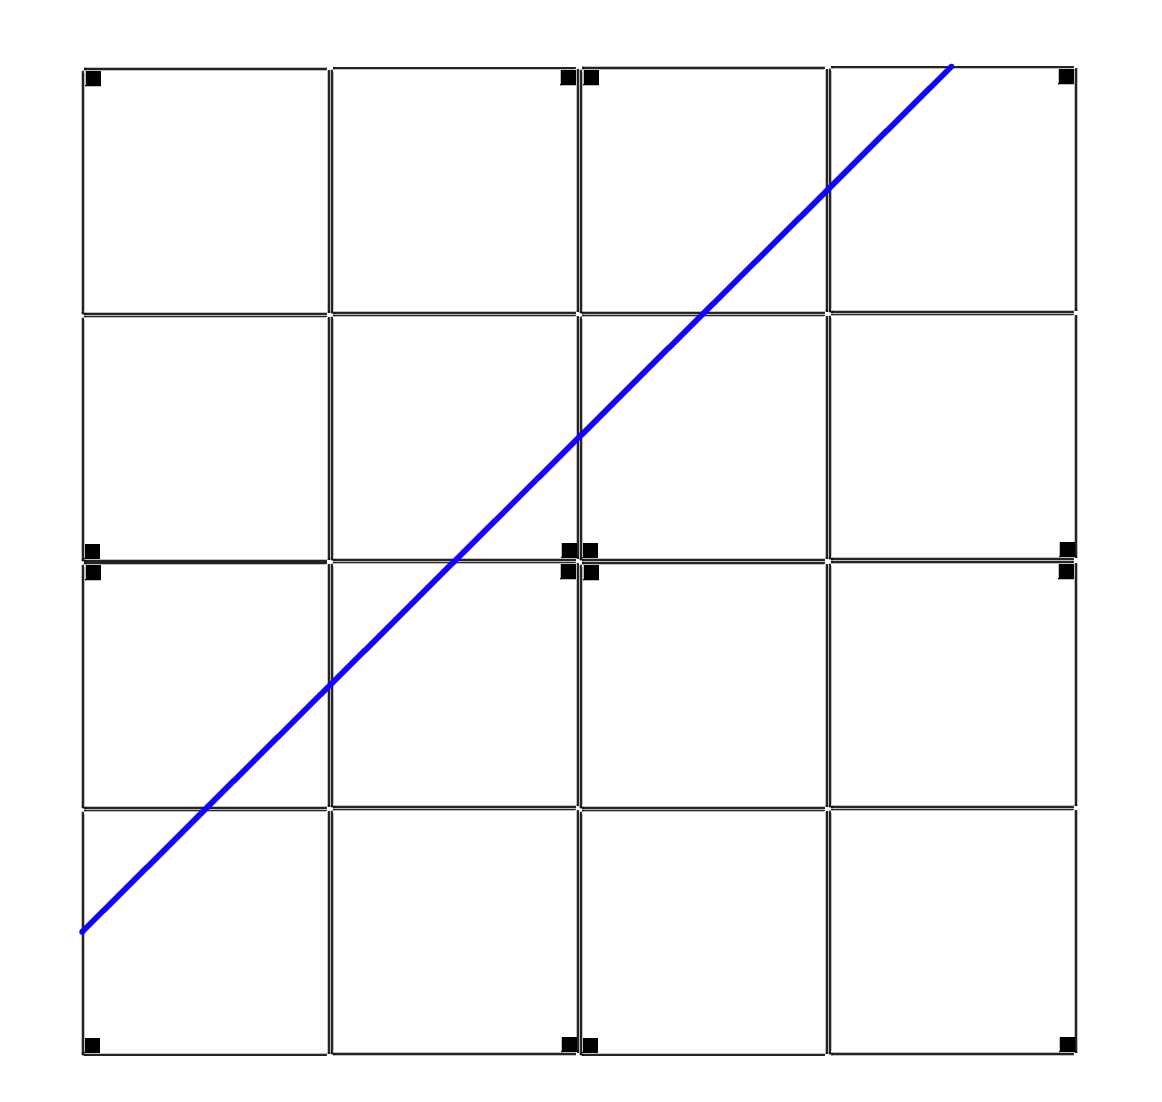
\includegraphics[width=3in]{tiling.png}
  \caption{\label{fig:tiling}Example of Tiling Billiard Tables}
\end{figure}

A couple of interesting observations can be made:

\begin{itemize}
  \item The combined trajectory $T = \{\tau(0, \kappa_1), \tau(\kappa_1, \kappa_2), \tau(\kappa_2, \kappa_3), \ldots \}$ of a ball creates a ray inthe $xy$ plane.
  \item $v$ collisions happen exactly when the combined trajectory $T$ intersects with the vertical lines $x = k$ where $k \in \mathrm{Z}$.
  \item $h$ collisions happen exactly when the combined trajectory $T$ intersects with the horizontal lines $y = k$ where $k \in \mathrm{Z}$.
\end{itemize}

\begin{theorem}
  The trajectory of a billiard ball is a ray in the $xy$ plane under the tiling representation.
\end{theorem}
